% 必需宏包：tikz、amssymb、array（若导言区尚未加载，请补充）

\begin{center}
    \textbf{\Large 河北工程大学 2024--2025 学年第二学期期末考试试卷（A）卷}
\end{center}

\setcounter{section}{0}

\section{单选题（每题 2 分，共 20 分）}

\begin{enumerate}
    \item 设 $N$ 是自然数集，$Z$ 是整数集，对于任意 $x\in Z$，令 $f: Z\to N$，$f(x)=|x|$，则 $f$ 是（\quad）。
    \choicelow{仅是单射}{仅是满射}{是双射}{不是函数}

    \item 设 $*$ 是 $A$ 上的 $2$ 元代数运算，若对于任意的 $x,y\in A$，均有 $x*y=y*x$，则称 $*$ 满足（\quad）。
    \choicelow{交换律}{结合律}{对合律}{分配律}

    \item 设二元关系 $R\in A\times A$，若对于任意 $x\in A$，均有 $(x,x)\in R$，则称 $R$ 是 $A$ 上的（\quad）。
    \choicelow{自反关系}{对称关系}{反对称关系}{传递关系}

    \item 以下不属于等价关系具有的性质是（\quad）。
    \choicelow{自反性}{对称性}{传递性}{反对称性}

    \item 在命题逻辑中，“如果 $p$，则 $q$”可以表示为 $p\to q$。那么，“$p$ 当且仅当 $q$”应表示为（\quad）。
    \choicelow{$p\land q$}{$p\lor q$}{$p\leftrightarrow q$}{$\neg p\lor q$}

    \item 逻辑等值于命题公式 $p\to q$ 的是（\quad）。
    \choicelow{$\neg p\land q$}{$\neg p\lor q$}{$p\lor \neg q$}{$p\leftrightarrow q$}

    \item 在谓词逻辑中，表示“存在至少一个 $x$ 使得 $P(x)$ 为真”的公式是（\quad）。
    \choicelow{$\exists x P(x)$}{$\forall x P(x)$}{$\exists x\neg P(x)$}{$\neg\exists x P(x)$}

    \item 谓词逻辑中的“论域”指的是（\quad）。
    \choicelow{谓词的定义域}{谓词的值域}{个体讨论的范围}{函词的定义域}

    \item 设 $G=(V,E)$ 是无向图，则 $G$ 是连通图当且仅当 $G$ 的连通分支 $w(G)$ 为（\quad）。
    \choicelow{$w(G)=1$}{$w(G)=2$}{$w(G)>2$}{$w(G)\geq 2$}

    \item 设 $G=(V,E)$ 是任意图，$G$ 中经过所有边一次且仅一次的路称为（\quad）。
    \choicelow{Hamiltonian 图}{Euler 图}{Hamiltonian 路}{Euler 路}
\end{enumerate}

\section{综合题（共 7 题，80 分）}

\begin{enumerate}
    \item 设有集合 $A=\{1,2,4,5,7\}$，$B=\{2,3,5,6\}$，全集 $U=\{1,2,3,4,5,6,7\}$。求 $A\cap B$、$A\cup B$、$\overline{A}$、$A-B$。（8 分）

    \vspace{3cm}

    \item 已知 $A=\{1,2,3,4\}$，$A$ 上的二元关系
    $R=\{(1,2),(3,4),(4,3)\}$，
    $S=\{(1,3),(3,4),(4,1)\}$，求出 $R\cap S$、$R\cup S$、$R^{-1}$、复合关系 $R\circ S$。（10 分）

    \vspace{3cm}

    \item 设 $A=\{1,2,3,4\}$，$A$ 上的关系
    $R=\{(1,2),(2,4),(3,3),(1,3)\}$，求出自反闭包 $r(R)$、对称闭包 $s(R)$ 和传递闭包 $t(R)$。（10 分）

    \vspace{3cm}

    \item 用真值表法求命题公式 $(\neg p\lor q)\to r$ 的主析取范式和主合取范式。（12 分）

    \vspace{3cm}

    \item 证明如下推理：
    $p\to(q\lor r)$，$\neg s\to \neg q$，$p\land \neg s\Rightarrow r$。（10 分）

    \vspace{3cm}

    \item 符号化如下命题并证明该推理有效性：所有有理数都是实数，有些有理数是整数，所以有些实数是整数。（15 分）

    \vspace{3cm}

    \item 使用 Dijkstra 算法求 $v_1$ 到其余各顶点的最短路径，以表格形式简化算法求解过程，并指出其中 $v_1$ 到 $v_6$ 的最短路径及长度。（15 分）

    \begin{center}
    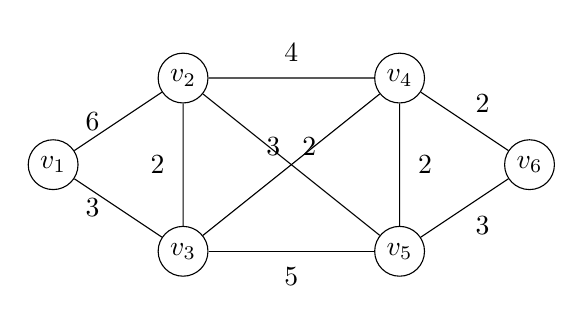
\begin{tikzpicture}[scale=1.1, every node/.style={circle, draw, inner sep=1.5pt, minimum size=18pt}]
        \node (v1) at (0,1) {$v_1$};
        \node (v2) at (1.5,2) {$v_2$};
        \node (v3) at (1.5,0) {$v_3$};
        \node (v4) at (4,2) {$v_4$};
        \node (v5) at (4,0) {$v_5$};
        \node (v6) at (5.5,1) {$v_6$};

        \draw (v1) -- node[draw=none, fill=none, left] {$6$} (v2);
        \draw (v1) -- node[draw=none, fill=none, left] {$3$} (v3);
        \draw (v2) -- node[draw=none, fill=none, left] {$2$} (v3);
        \draw (v2) -- node[draw=none, fill=none, above] {$4$} (v4);
        \draw (v3) -- node[draw=none, fill=none, below] {$5$} (v5);
        \draw (v4) -- node[draw=none, fill=none, right] {$2$} (v5);
        \draw (v4) -- node[draw=none, fill=none, above right] {$2$} (v6);
        \draw (v5) -- node[draw=none, fill=none, below right] {$3$} (v6);
        \draw (v2) -- node[draw=none, fill=none, above right] {$2$} (v5);
        \draw (v3) -- node[draw=none, fill=none, above left] {$3$} (v4);
    \end{tikzpicture}
    \end{center}

    \vspace{3cm}
\end{enumerate}